\chapter{Conclusions and Future Work}
\label{ch:conclude}
This dissertation presents a new approach to perform reachability
analysis of FSMs at the word-level. It is facilitated by investigating the analog of 
implicit state enumeration algorithm in computer algebra and algebraic
geometry domains. The image function part of the computation is mapped to a variety projection on 
next state variables. This projection is implemented by computing the 
Gr\"obner basis of an elimination ideal with abstraction term orders.
Moreover, the set operations in the state space are mapped to 
the arithmetic of ideals, as algebraic geometry provides a 
way to reason about the variety (solutions) by manipulating the ideals.
A special term order (RATO) is utilized to improve the Gr\"obner bases 
computation, and a tool is developed to implement our 
word-level FSM traversal algorithm. Experiments are performed to 
analyze the reachability for ISCAS'89 and ITC'99 circuit benchmarks.

Next, we describe a method to execute functional verification on sequential Galois field
multipliers over $\Fkk$.  The core algorithm is based on word-level unrolling of 
a Moore machine, which applies concepts from the word-level FSM traversal 
algorithm. As a result, transition relations are represented 
as a polynomial with word-level inputs/outputs.
We implement our algorithm with both the \textsc{Singular} platform and a custom C++ toolset 
and perform experiments on two classes of circuits.
Our approach is able to verify up to 162-bit sequential
circuits, whereas contemporary techniques fail beyond 23-bit
datapaths.  

At last we explore abstraction UNSAT cores in algebraic geometry -- the foundation for refinement techniques
to boost sequential circuit verification.
% UNSAT core extraction, as an indispensable component of many refinement algorithms 
% which rely on UNSAT informations, is thus proposed in polynomial rings.
We use the Weak Nullstellensatz as the essential theory of UNSAT core extraction, 
then develop heuristics to improve the core that exploit the structure of the refutation proof.
An algorithm was implemented within the \textsc{Singular} computer algebra tool
and experiments were conducted to validate the approach.

Our approaches still have limitations: for word-level FSM traversal and 
sequential GF multiplier verification, our methods are more efficient
for XOR-rich circuits, while most industrial designs are AND-OR gate dominant.
For UNSAT core extraction, the abstraction refinement approach such as $k$-BMC 
has only limited application on certain model checking problems. To overcome these limitations,
the following further explorations are worthy of investigation. 
  
\section{Future Work}
In this section, we highlight some research problems that deserve further study.
\subsection{Multivariate Polynomial Ideal based FSM Traversal}
In Chapter \ref{ch:reacha}, we always use a single word-level variable $T$ to denote the
next state. However, in some situations we need to keep recording the relations between $T$ and
inputs, {\it i.e.} the reached states contain multivariate polynomials in $T,S$ and PI $x$. 
While the elimination and set union/intersection are compatible with multiple NS variables,
the set complement requires an extension of Theorem \ref{thm:quotient} on ideals with 
multivariate polynomial generators. We conjecture as follows:

\begin{Conjecture}
Assume we are given ring variables $x_i$, and an ideal $J$ composed by $s$ generators:
$J = \langle f_1,\dots, f_s\rangle$.  Additionally $J_0$ is the vanishing polynomial for variables
$x_i$: $ x_i^{q} - x_i$ where $q$ is the size of signal $x_i$ represents.
We conjecture that
$$V(J') = V(J_0:J) = V(J_0)\setminus V(J) = \overline{V(J)}$$
% And we believe this conjecture is scalable such that it is also valid for even more variables and generators like 
% $J = \langle f_z, v_x,v_y,v_u,v_w\rangle$, $f_z =\mathcal F (z,x,y,u,w)$.
\end{Conjecture}

In univariate case, $\F[x]$ is the principle ideal domain thus Theorem \ref{thm:quotient} can be proved.
However over multivariate case, the proof of this conjecture is not available.
% 
% The following example illustrates a different operation from Example \ref{ex:SMPO}.
% \begin{Example}
% In Figure \ref{fig:fsm}
% $\{s_0, s_1\}$ are state/pseudo inputs, $\{t_0,t_1\}$ are state/pseudo outputs, and there is a primary input (1-bit) 
% $x$. We propose a new algorithm by modifying Algorithm \ref{alg:univa}:
% 
% \IncMargin{1em}
% \begin{algorithm}[hbt]
% \SetAlgoNoLine
% \LinesNumbered
%  \KwIn{Transition polynomial $f_t = T + \mathcal F (S,x)$, 
% 	initial state ideal $from^0 = \langle S+\mathcal G(x), x^{q_1} - x\rangle$}
%  \KwOut{Reachable states}
%   $reached = from^0(T\setminus S)$\;
%   \Repeat{$GB(new^i) == 1$}
%   {
%   	$i \gets i + 1$\;
% 	$to^i \gets$GB$(\langle f_t, from^{i-1}\rangle) \setminus \mathcal H(S)$\;
% 	$\overline{reached} = \langle T^{q_2}-T, x^{q_1} - x \rangle : reached$\;
% 	$new^i \gets $GB$(to^i + \overline{reached})$\;
%   	$reached \gets $GB$( reached \cdot new^i)$\;
% 	$from^i \gets new^i(S\setminus T)$\;
%   }
% \Return{$reached$}
% \caption {Algebraic Geometry based Traversal Algorithm (multivariate-generator ideals)}\label{alg:multi}
% \end{algorithm}
% \DecMargin{1em}
% 
% The inputs of this algorithm includes transition polynomial (result of word-level abstraction) and initial 
% states description ideal, which contains 2 generators corresponds to constraints of PI and combinational input $S$. 
% For example, $\langle S+1+\alpha, x^2+x\rangle$ means initial state$=\{11\}$,
% $\langle S+x\cdot\alpha, x^2+x\rangle$ means initial states$=\{00,10\}$).
% 
% Transition polynomial calculation uses the abstraction and bit-to-level conversion method from 
% Chapter \ref{ch:reacha}. After Constructing
% an elimination ideal, we impose RATO such that \emph{reverse\ topo\ order\ ckt\ variables }$> T > S > x$, the reduction
% remainder has the form $T+\mathcal F(s_0,s_1,x)$. From word definition $S+s_0+s_1\alpha$ we get
% $$s_0 = \alpha S^2+ (1+\alpha)S, s_1 = S^2+S$$
% Do substitution, the transition polynomial of example ckt is 
% $$f_T = T+S^3\cdot x+\alpha S^3+(1+\alpha)S^2\cdot x+S^2+S\cdot x+(1+\alpha)x+1$$
% 
% Assume we start from state $\{11\}$. In the first iteration, the reached state is $\{01\}$. Line 4 is to compose an
% ideal with 2 generators from $from^0$ and transition polynomial $f_T$, compute its Gr\"obner basis. Note this ideal
% has the form
% \begin{equation}
% I_{tran} = \left\{
%              \begin{array}{c}
%              T+\mathcal F(S,x) \\
%              S + \mathcal G(x) \\
%              v_x
%              \end{array}  
%         \right.
% \end {equation}
% $v_x$ is a polynomial containing only $q$-bit PI $x$, initially it should be vanishing polynomial $x^{q_1}-x$, 
% with the program executing it may be factorized.
% 
% Consider Buchberger's algorithm, all generators' leading terms are relatively prime, so it is a GB itself. 
% Then we need to reduce this GB, we will find out $S + \mathcal G(x)$ could (possibly) be reduced by $v_x$,
% and $T+\mathcal F(S,x)$ will definitely reduced by $S + \mathcal G(x)$. So, at last we will get a polynomial
% $T + \mathcal F'(x)$ in reduce GB. We can include this polynomial and $v_x$, exclude the polynomial containing
% $S$ (i.e. $\mathcal H(S)$ in algorithm), to compose an ideal representing \emph{next states} $to^i$. 
% In iteration 1, result is $to^1 = \langle T+1, x^2+x\rangle$
% 
% Line 5 is the ideal quotient of universal set and reached states. In the first iteration, 
% $reached$ is the initial state $\langle T+1+\alpha, x^2+x \rangle$. Result of ideal quotient
% is $\langle T^3+(1+\alpha)T^2+\alpha T, x^2+x\rangle$ represents $\{00,01,10\}$.
% 
% Line 6 is ideals' sum (intersection of their varieties), it is done by combining all generators
% from 2 ideals and compute GB. For first iteration result is $GB(\langle T+1,T^3+(1+\alpha)T^2+\alpha T, x^2+x\rangle) = \langle T+1, x^2+x\rangle$ representing $\{01\}$.
% 
% Line 7 is ideals' product (union of their varieties), it is done by multiplying all pairs of
% generators from both ideal. For first iteration result is $GB(\langle (T+1)(T+1+\alpha),
% (T+1)(x^2+x), (T+1+\alpha)(x^2+x), (x^4+x)\rangle) = \langle T^2+\alpha T+(1+\alpha), x^2+x\rangle$ representing $\{01,11\}$.
% 
% The traversal will run 3 iterations and terminate at 4th iteration. I list all intermediate 
% results below:
% \begin{itemize}
% \item Iteration 1: $from^0 = \langle S+1+\alpha, x^2+x\rangle, to^1 = \langle T+1, x^2+x\rangle,
%  reached = \langle T^2+\alpha T+(1+\alpha), x^2+x\rangle$
% \item Iteration 2: $from^1 = \langle S+1, x^2+x\rangle, to^2= \langle T+\alpha, x^2+x\rangle,
% reached = \langle T^3+1, x^2+x\rangle$
% \item Iteration 3: $from^2 = \langle S+\alpha, x^2+x\rangle, to^3 = \langle T+\alpha x, x^2+x
% \rangle, reached = \langle T^3\cdot x+x, T^4+T, x^2+x\rangle$
% \item Iteration 4: $from^3 = \langle S, x\rangle, to^4 = \langle T+1, x\rangle, new = \langle1\rangle$
% \end{itemize}
% The final reachable states are represented by multivariate polynomial ideal $\langle T^3\cdot x+x, T^4+T, x^2+x\rangle$,
% which denotes $\{00,01,10,11\}$.
% \end{Example}

\subsection{Use of the $F_4$ Algorithm and ZDDs to Accelerate GB Reduction}
In Chapters \ref{ch:reacha} and \ref{ch:normal}, by using RATO we transform the GB-based
computation to that of a multivariate polynomial division. However, this division (reduction)
still incurs exponential complexity in the worst case. In a situation where division is to be performed modulo
a chain of OR gates, the size of remainder polynomial will explode. For example, a chain of OR gates 
can be written as the Boolean function 
\begin{equation}
\label{eqn:chainOR}
f = ((a\lor b) \lor c) \lor d
\end{equation}
which equals to the following polynomial function in $\F_2$:
$$f = abcd+abc+abd+ab+acd+ac+ad+a+bcd+bc+bd+b+cd+c+d$$
Notice, $f$ contains $2^4-1 = 15$ terms, which is exponential in the number of variables.
The size explosion is a major factor affecting the efficiency of polynomial division.

One way to further boost the efficiency is to adopt techniques from sparse linear algebra.
Analysis of experimental results shows that multivariate polynomial division procedure
consumes most of the verification time.
A matrix-based technique named as "$F_4$ style reduction" \cite{f4} can speed up the procedure of
dividing a low-degree polynomial with a term-sparse polynomial ideal. 

Another way is to utilize DDs, {\it e.g.} ZDDs. ZDDs can represent unate covers of Boolean formulas.
We can represent $f$ using a ZDD, where every path in the ZDD from a root to a terminal corresponds
to a monomial term.

\begin{figure}[h]
\centerline{
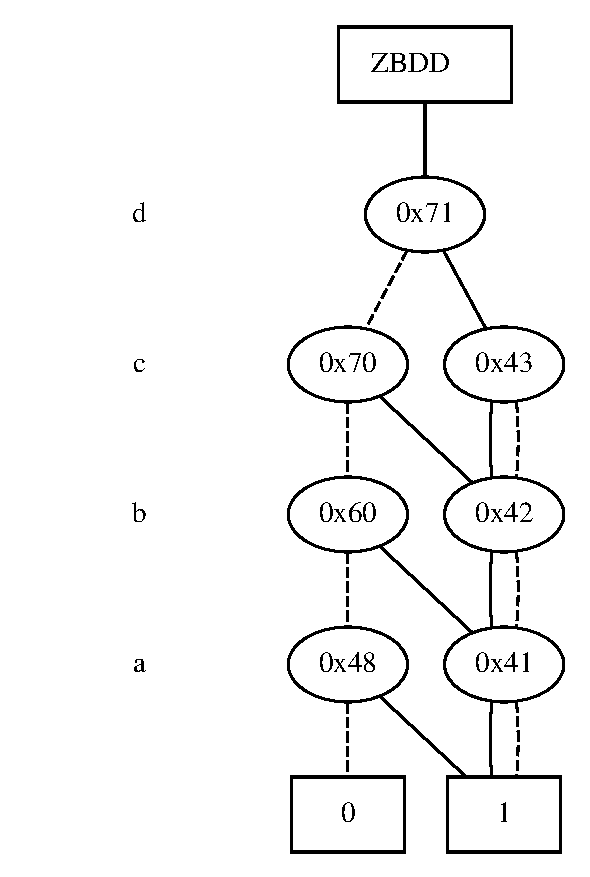
\includegraphics[width=0.35\textwidth]{newfig/ZDD.eps}
}
\caption{A ZDD representing remainder polynomial reducing by a chain of OR gates with order $d>c>b>a$}
\label{fig:ZDD}
\end{figure}

Figure \ref{fig:ZDD} shows a ZDD representing 
Equation \ref{eqn:chainOR} with size $2\times4 -1 = 7$, which is linear in the number of variables.
The reduction process using ZDDs can be executed as in \cite{polybori:2009}. The graphical illustration 
of the remainder in ZDDs is also shown in Figure \ref{fig:ZDD}. 

\subsection{Craig Interpolants in Algebraic Geometry}
The concept of Craig Interpolants (CI) and their existence comes from
symbolic logic \cite{craig-interpolate}; later, algorithms were
presented to find the CI for Boolean formulae
\cite{pudlak:ci} \cite{mcmillan2003interpolation}. Assume that Boolean
formulae are represented in Clause Normal Form (CNF) as 
$f = C_1 \wedge C_2 \wedge \dots \wedge C_m$ where: 1) Each clause
$C_i$ is a disjunction (Boolean OR, denoted $\vee$) of literals; 2)
Each literal is a Boolean variable $x_i$ or its complement
$\overline{x_i}$. 
The Boolean satisfiability (SAT) problem requires that we find an
assignment to the variables such that the formula $f$ is satisfied
(SAT), or otherwise prove that no such assignment exists (UNSAT). 
A CI is related to an UNSAT formula. 

\begin{Definition}
(From \cite{mcmillan2003interpolation}) Let $A$ and $B$ be Boolean
  formulas given as sets of clauses such that $A \wedge B$ is
  unsatisfiable (UNSAT). Then there exists a formula $P$ such that: 
1) $A$ implies $P$ (or $A \subseteq P$); ~2) $P \wedge B$ is UNSAT; ~3)
$P$ refers to only the common variables of $A$ and $B$. The formula
$P$ represents an {\bf interpolant} of $A$ and $B$. 

Given  the pair $(A, B)$ and their refutation proof, a procedure
called interpolation system constructs an interpolant in linear time
and space in the size of the proof \cite{mcmillan2003interpolation}
\cite{pudlak:ci}. 
\end{Definition}

\begin{Example}\label{ex1}
Let $f = (\overline{d})(\overline{c})(\overline{a}\vee d)(a
\vee b \vee c)(\overline{b})$ be a CNF formula. Let $f = A \wedge B =
\emptyset$, where $A = (\overline{d})(\overline{c})(\overline{a}\vee
d)$ and  $B = (a \vee b \vee c)(\overline{b})$. Then $P = \overline{a}
\wedge \overline{c}$ is an interpolant of $(A, B)$. 
\end{Example}

CIs are used to derive abstractions to produce over-approximate image
operators in model checking \cite{mcmillan2003interpolation}. Since $A
\implies P$, $P$ contains $A$ and is an {\it abstraction} of $A$. It
also has fewer variables, so checking  invariants on $P \wedge B$ is
easier. The interpolant is derived through a resolution proof of the
SAT problem. There can be many interpolants $P_i$ for a pair $(A,B)$; 
however, it is not feasible to explore a few or all of these
interpolants by means of the resolution proof. 


We introduce the algebraic geometry analog of CI.
We conjecture that the
  concept of CI should be related to elimination ideals, so future lines
  of investigation should focus on \Grobner basis computations with
  elimination term orders for their computation.



\begin{Definition}\label{ci}
Let $F = \{f_1, \dots, f_s\}$ be a set of polynomials in the ring 
$R = \Fq[x_1,\dots,x_n]$. Let $F = F_A \cup F_B$ and ideals $J =
\langle F \rangle, J_A = \langle F_A \rangle, J_B = \langle F_B
\rangle$ be corresponding ideals in $R$ such that $J = J_A + J_B$. Let
it be known (say, due to application of Weak Nullstellensatz and
Gr\"obner basis) that the varieties $V_{\Fq}(J) = V_{\Fq}(J_A) \cap
V_{\Fq}(J_B) =V_{\Fq}(J_A+J_B)=\emptyset$. Also, let the set of
variables $X = \{x_1,\dots,x_n\} = X_A \cup X_c \cup X_B$ where $X_A,
X_B$ are the set of variables present exclusively in the sets of
polynomials $F_A, F_B$ respectively. Only $X_c$ is the set of
variables that are common to both sets of polynomials $F_A,
F_B$. Then, there exists a set of polynomials  $F_P$ and ideal $J_P =
\langle F_P \rangle$ such that 
\bi
\item $V_{\Fq}(J_A) \subseteq V_{\Fq}(J_P)$
\item $V_{\Fq}(J_P) \cap V_{\Fq}(J_B) = \emptyset$
\item Polynomials of $F_P$ contain the common variables ($X_C$) of
  $F_A, F_B$. 
\ei

We call the ideal $J_P = \langle F_P\rangle$ the {\bf algebraic
  interpolant} of  $J_A+J_B$. 
\end{Definition}

Existence of algebraic interpolant comes from \cite{craig-interpolate}.
The question for exploring is that how do we compute it in algebraic geometry?

\begin{Example} \label{ex2}
Based on Example \ref{ex1}, we translated the system over
$\mathbb{F}_2[a, b, c, d]$. Let $F_A = \{f_1, f_2, f_3\}$ and $F_B =
\{f_4, f_5\}$ where: $f_1: d; ~~~f_2: c; ~~~f_3: a + da; f_4:  abc +
ab + ac + bc + a + b + c + 1; ~~~f_5: b.$ The Boolean interpolant
$\overline{a}\wedge\overline{c}$ from Example \ref{ex1} translates to
${\mathbb{F}}_2$ as the polynomial $f_p = ac + a + c$, with its
variety $V(f_p) = \{a=0, c=0\}$.   
\end{Example}

% {\bf Research problem 2:}
% {\it How can this algebraic interpolant $f_p$ (or in the general case,
%   the set of polynomials $F_P$) be computed? As the interpolant $F_P$ 
% contains only variables $X_C$ that are common to the polynomial sets
% $F_A, F_B$, does this imply that the interpolants can be computed by
% means of \Grobner bases with an elimination term order $X_A>X_B>X_C$
% with $X_A, X_B$ eliminated from the problem? }

Algebraic interpolation is strongly related
to the GB computation with the elimination order $X_A>X_B>X_C$, and
this relationship needs to be formally derived. 

\begin{Conjecture} \label{con:ci}
Computations of algebraic interpolants: Let $J_0$ denote the ideal of
all vanishing polynomials in $\Fkk[x_1,\dots,x_n]$.
\bi
\item  Compute a Gr\"obner basis $G_1 = GB(J_A + J_0)$ 
with the elimination order $X_A > X_B > X_C$, and select
$F_{P1}=G_1\cap\Fkk[X_C]$. We conjecture that the \Grobner
basis $F_{P1}$ of the elimination ideal corresponds to an algebraic
interpolant. 

\item Analogously, compute a Gr\"obner basis $G_2 = GB(J_B + J_0)$ 
with the elimination order $X_B > X_A > X_C$, and select
$F_{P2}=G_2\cap\Fkk[X_C]$. Find an ideal $F'_{P2}$ such that
the variety $V(F'_{P2})$ is the complement of the variety
$V(F_{P2})$. Then the set $F'_{P2}$ gives another interpolant.
\ei
\end{Conjecture}


\begin{Example}\label{ex3}
Consider the polynomials $\{f_1, \dots,f_5\}$ from Example
\ref{ex2}. Computing $F_{P1}$ as described in Conjecture \ref{con:ci} 
produces $F_{P1} = \{a, c\}$, correctly giving us the desired variety
$V(a = 0, c = 0)$. Similarly, when we compute $F_{P2}$, we find that
the interpolant is $ac + a + c + 1$. Notice that the variety 
$V(ac+a+c+1)=\{(0,1), (1,0), (1,1)\}$, which is exactly the complement
of $V(F_{P1})$.  
\end{Example}

The aforementioned experiments in Example \ref{ex3} do not invalidate
our conjectures. Moreover, the above experiment shows that there can be
multiple ways of computing the interpolants. What can these \Grobner
basis computations tell us about the number of valid algebraic
interpolants for any given problem? Can they be classified as {\it weak
  or strong interpolants} based on the sparsity of the polynomials
(power of abstraction)? 

As there can be many interpolants for an ideal-pair $(J_A, J_B)$, 
the following questions should also be investigated in the future:
\bi
\item Find the minimal interpolant: {\it i.e.} find the interpolant $F_P$
  such that $V(J_P)$ is the smallest variety larger than $V(J_A)$ such
  that $V(J_P) \cap V(J_B) = \emptyset$.
\item Analogously, find the maximal interpolant. 
\item Over finite fields, the variety of an elimination ideal is
  exactly equal to the projection of the variety on the remaining
  variables. Consider Figure \ref{fig:projection}, where variety of the
  ideals $J_A, J_B$ are respectively projected on the common variables
  $X_C = \{a, c\}$. Then, does computing $F_{P1}$ (resp. $F_{P2}$) 
  deliver the minimal (resp. maximal) interpolant?
\ei

\begin{figure}[h]
\centering{
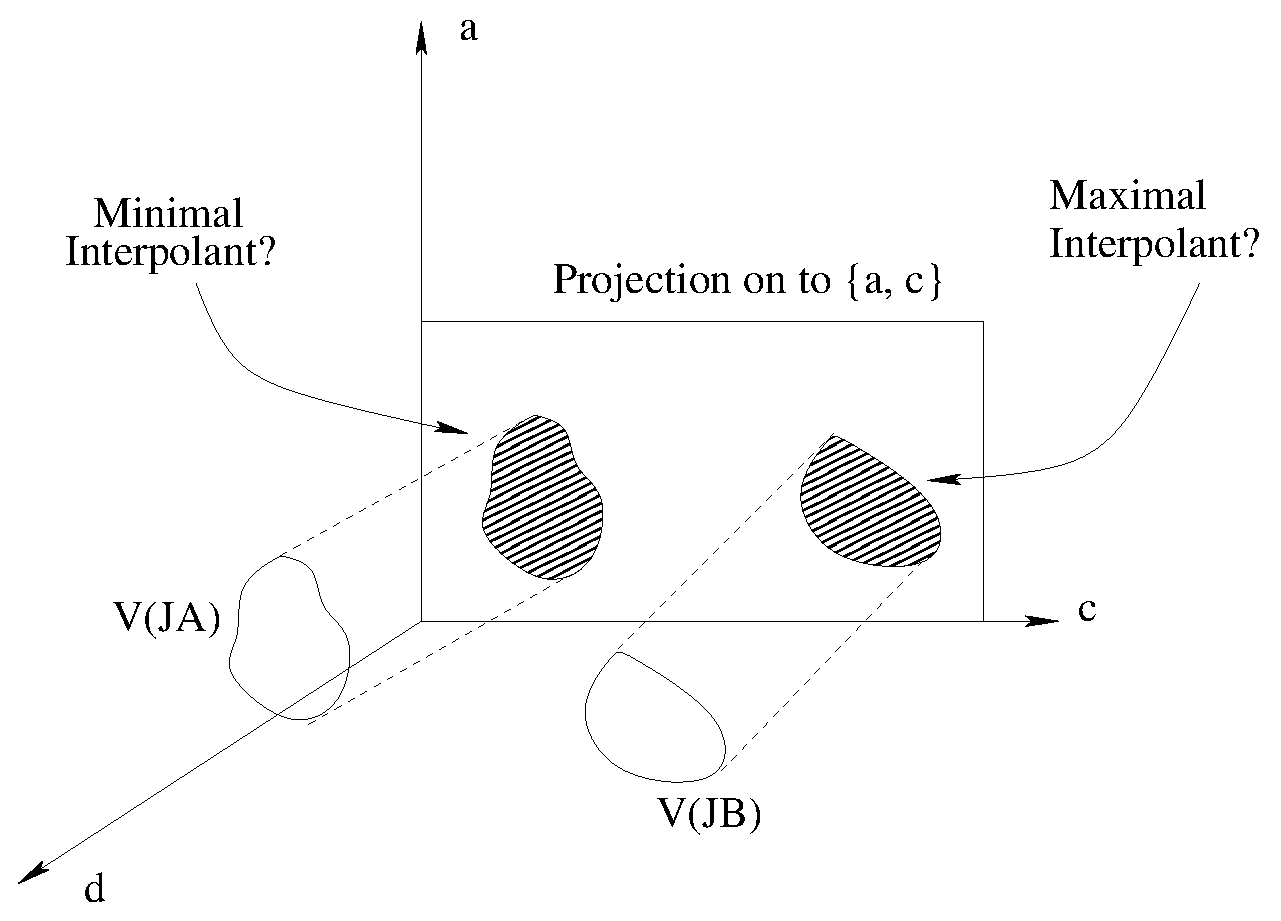
\includegraphics[width=4.5in]{newfig/project.eps}
\caption{Algebraic interpolant: Projection of varieties on common variables? }
\label{fig:projection}}
\end{figure}

% 
% Once these problems are understood and algorithms for the computation
% of algebraic interpolants derived, then we will integrate them 
% with word-level reachability analysis for abstraction-based model
% checking. 

% \subsection{Technology Mapping for Word-level Functional Blocks}
% Technology mapping is an important problem in digital circuit synthesis.
% Designers are given a library of well-designed functional/macro blocks (including IP cores) and a raw netlist, 
% technology mapping's objective is to map as many as blocks to the raw netlist and 
% keep the functional equivalence. Contemporary techniques rely on bit-wise 
% analysis on the signals to deduce the boundary of mapped blocks.
% It is possible to use the equivalence checking techniques proposed in this dissertation 
% as a alternative way to perform technology mapping, especially on word-level when 
% given blocks represent word-level functions.
% 
% \begin{Problem}
% The objective of our approach is to map the macro blocks without boundary information.
% Mapping is an essential technique used in synthesis and verification. In synthesis, we can map the 
% macro functions with smaller and faster implementations to optimize the timing and area; in simulation,
% we can map a complicated function to a simple execution to accelerate simulation speed.
% 
% Given a gate-level design $D$ and several word-level macro blocks $\{B_i\}$, we need to map macro
% blocks $B_i$ into design $D$, and write out the mapped design $D'$ which is equivalent to original
% design $D$. The objective is to generate a mapped design $D$ with as many of $B_i$ such that the area
% and timing is optimal. The procedure is also illustrated in Figure \ref{fig:macro}.
% 
% \begin{figure}[h]
% 	\begin{center}
% 	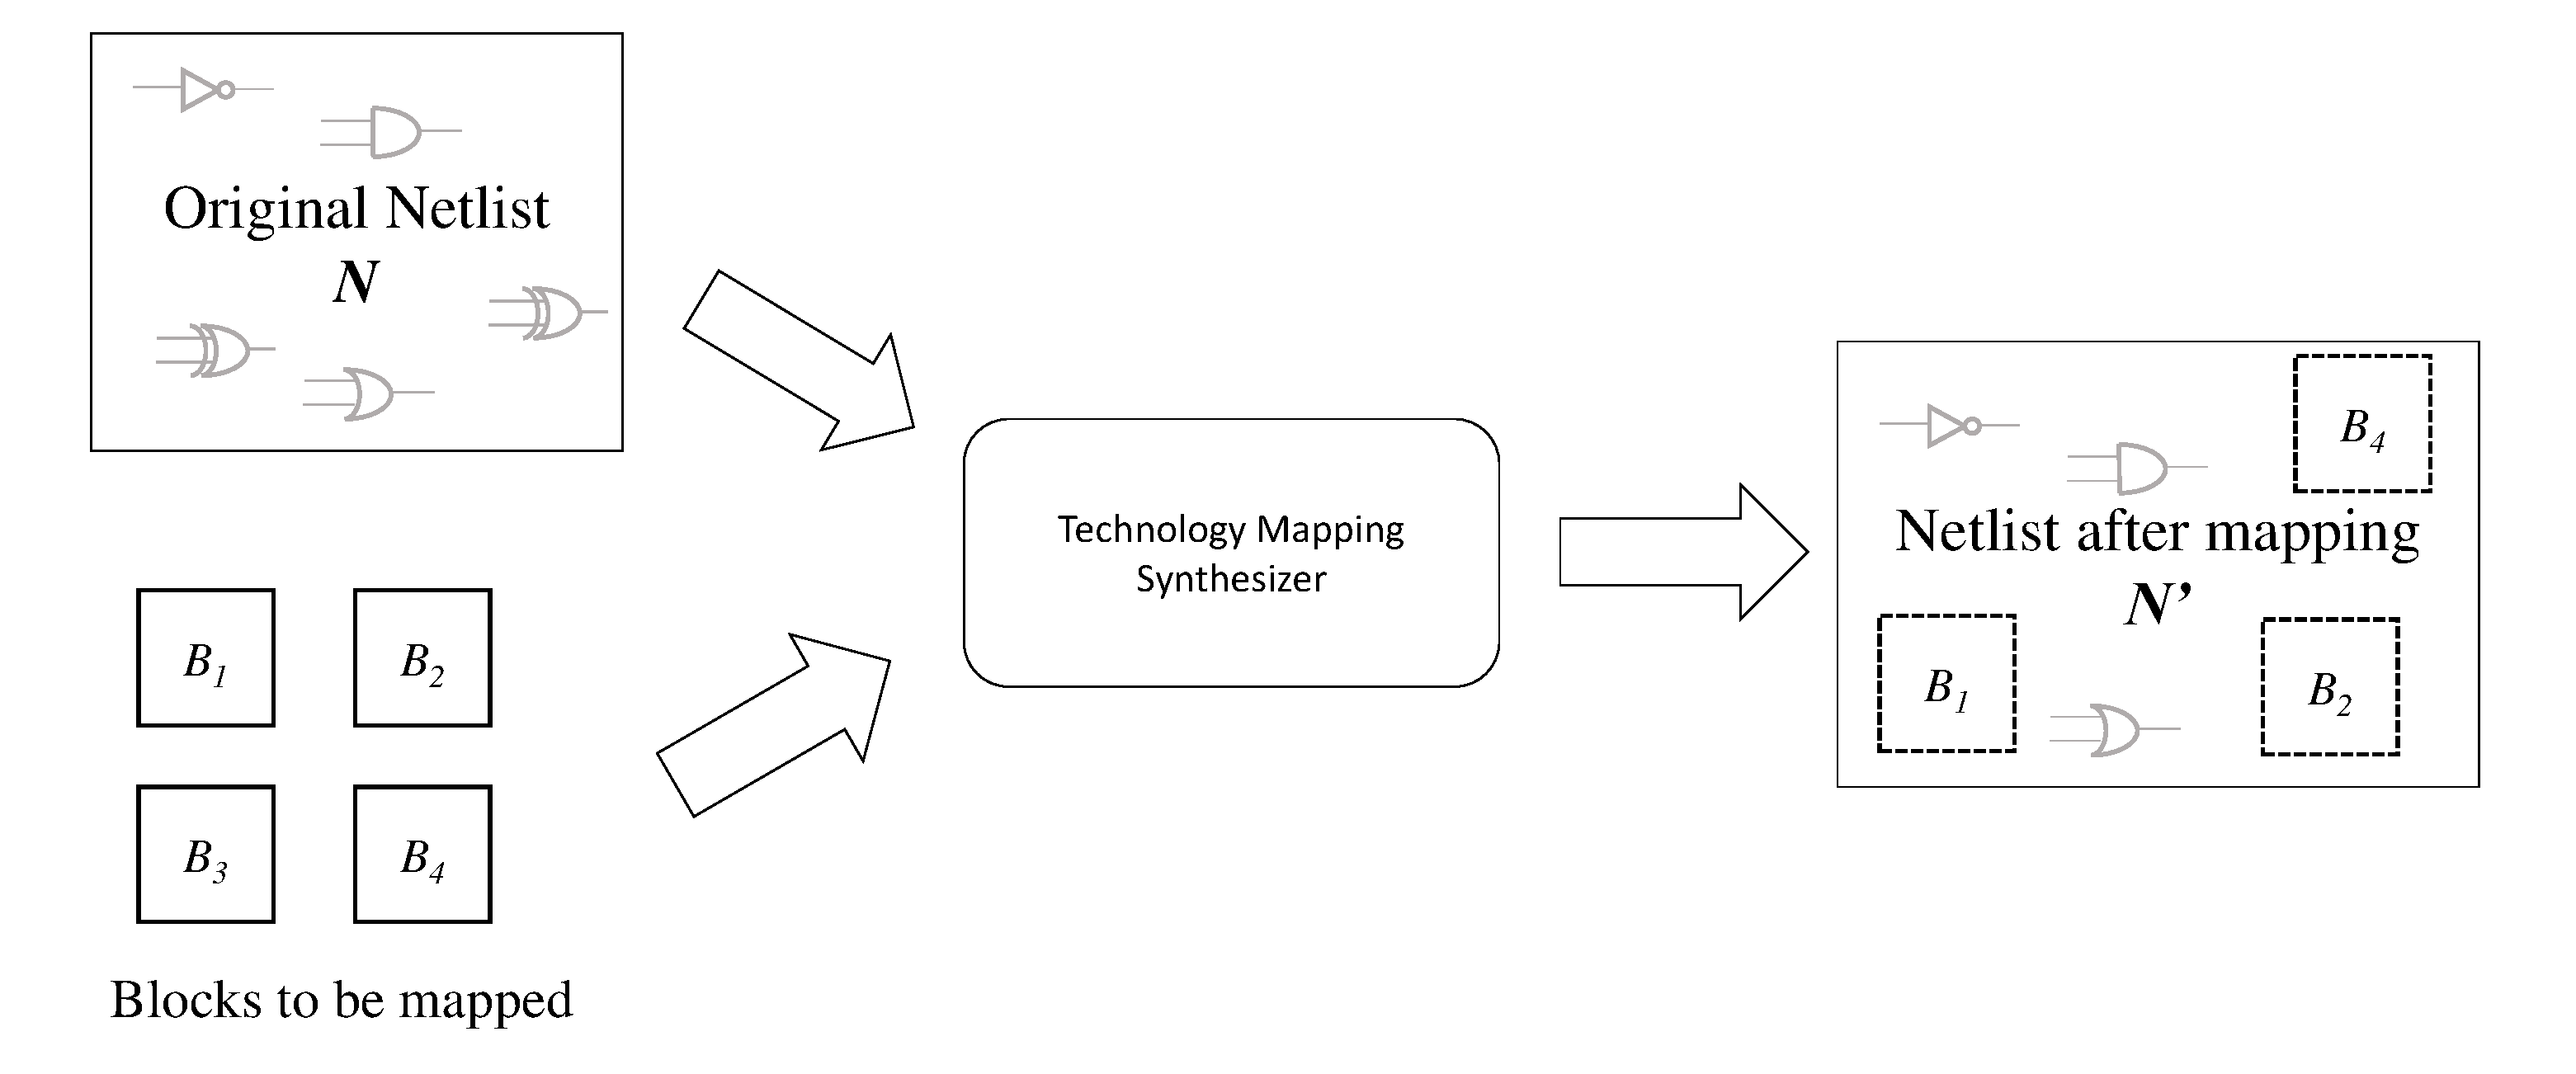
\includegraphics[width=\textwidth]{newfig/macro.pdf}
% 	\end{center}
% 	\caption{The outline and flow of technology mapping of macro blocks}
% 	\label{fig:macro}
% \end{figure}
% 
% \end{Problem}
% 
% The following part describes the sketch of our proposed approach base on loop invariant constraints \cite{sankaranarayanan2004non}.
% First, a transition system is modeled by algebraic assertions; then \emph{ideal membership test} \cite{lv:phd}
% is applied on the set of assertions to help abstract the loop invariant. We introduce concept \emph{template}
% from \cite{sankaranarayanan2004non} to apply on our proposed approach.
% 
% 1) {\bf Template and state constraints:}  Ideal membership test technique requires a setup of ideal $J_{loop}$
% for loop invariants. 
% One heuristic can provide better coverage for loop invariant abstraction as well as
% relatively small size is \emph{generic quadratic form} (GQF).
% 
% For example, the GQF of a pair of state variables $\{x,y\}$ is
% $$\Func = a_0x^2+a_1x+a_2xy+a_3y+a_4y^2+a_5$$
% It covers all possible terms with degree no more than 2. $a_0,a_1,\dots, a_5$ are usually real number parameters,
% some of their assignments can turn $\Func$ into desired invariant. This parameterized constrain
% polynomial covers all combinations of state variables can also be called a \emph{template}.
% Subsequently, finding a proper assignment is the essential part of in our proposed research.
% 
% 2) {\bf Initial state constraints:} For initial states, the constrains are explicit. A template is adopted and refined by Gr\"obner basis 
% generated by original constrains, by equaling the remainder to 0 we can get constrains on
% parameters from the template.
% 
% An example is shown in the following 3-line algorithm multiplying two natural numbers. 
% \begin{align}
% \label{eqn:loopinv}
% & {\bf integer}~~i,j,s~~{\bf where}(s=0 \land j=j_0) \nonumber\\
% & l_0: {\bf while}~~(\cdots)~~{\bf do} \nonumber\\
% & ~~~~ l_1:~(s,j)\gets(s+i,j-1) 
% \end{align}
% 
% Its template is generic quadratic form of $\{s,i,j,j_0\}$, which is
% \begin{align}
% \Func = & a_0s^2+a_1s+a_2si+a_3sj+a_4sj_0\nonumber\\
% &a_5i^2+a_6i+a_7ij+a_8ij_0+a_9j^2\nonumber\\
% &a_{10}j+a_{11}jj_0+a_{12}j_0^2+a_{13}j_0+a_{14}\nonumber
% \end{align}
% with parameters $a_0,\dots,a_{14}$.
% 
% Constrains of initial state $s=0\land j=j_0$ can be interpreted to polynomials:
% $$\{s, j-j_0\}$$
% Since their leading terms are relatively prime, the polynomial set itself constitutes a Gr\"obner basis 
% $$G=\{s, j-j_0\}$$ 
% Therefore its ideal can be written as
% $J=\langle s,j-j_0\rangle$.
% 
% In the next step, we reduce the template with the Gr\"obner basis $G$: $\Func \xrightarrow{G}_+ r$, the remainder equals to
% $$r = a_5i^2+a_6i+(a_7+a_8)ij_0+(a_9+a_{11}+a_{12})j_0^2+(a_{10}+a_{13})j_0+a_{14}$$
% Let it equal to 0, then each coefficient will generate a constraint. The solution to the system forms the candidate
% assignment to generate loop invariants.
% \begin{equation}
% \left\{
% \begin{array}{l}
% a_5=a_6=a_{14}=0\\
% a_7+a_8=0\\
% a_9+a_{11}+a_{12}=0\\
% a_{10}+a_{13}=0
% \end{array}\right.
% \nonumber
% \end{equation}
% 
% 3) {\bf Modeling state transitions:}
% A typical state transition starts from the previous state (PS) and ends at next state (NS). 
% Our proposed approach models the 2 states individually,
% {i.e.} performs polynomial reduction separately and obtains remainder $r_1$ and $r_2$. 
% Assume a constraint polynomial describing
% the state transition is $r_t$, then we require that when invariant of PS holds and transition $PS \to NS$ stands,
% invariant of NS should also be satisfied:
% $$(r_1 = 0)\land (r_t = 0) \implies (r_2 = 0)$$
% One reasonable conjecture is
% $$r_t = r_1 - \lambda r_2$$
% Theoretically $\lambda$ can be any polynomial in arbitrary rings. To make it practical solving the system, 
% we limit $\lambda$ to the polynomial ring with only real numbers.
% 
% We take Equation \ref{eqn:loopinv} as the example (which refers to Example 10 in \cite{sankaranarayanan2004non}). 
% PS is initial state we just characterized 
% $$\Func = f(s,i,j,j_0)$$ 
% and NS has exactly the same form of constraint:
% $$\Func' = f(s',i',j',j_0')$$
% Considering the transition relation, we substitute $s'$ with $s+i$ and replace $j'$
% with $j-1$, $i'$ for $i$, $j_0'$ for $j_0$, respectively. 
% The template for NS is polynomial $f'$ in Example 10 in \cite{sankaranarayanan2004non}.
% 
% We then perform reduction with the Gr\"obner basis generated from the transition relation modeling, 
% and record its remainder $r_2$.
% From equality $r_2 = \lambda r_1$, we get constraints for the parameters. Solve the system using 
% similar algorithm to solve binate covering problems
% which is also described in Section 4 as \emph{elimination by splitting} technique in \cite{sankaranarayanan2004non}. 
% One branching result is:
% \begin{align*}
% &a_0,a_2,\dots, a_6, a_9,\dots,a_{14}=  0\\ 
% &a_1=a_7=-a_8
% \end{align*}
% The reduced remainder is: 
% $$r_2 = a_1s +(a_1-a_7)i+a_7ij+a_8ij_0 = a_1(s+ij-ij_0) = 0$$
% Thus the invariant of the program in Equation \ref{eqn:loopinv} is:
% $$s = i(j_0- j)$$
% We can verify the invariant by executing the program which calculates $i\times j_0$. 
% Initially $s=0$, $j_0-j=0$, invariant holds;
% during each cycle, $s'=s+i, (j_0'-j') = (j_0-j)+1$, the invariant also holds. In conclusion, this is a
% loop invariant for program in Equation \ref{eqn:loopinv}.
% 
% {\bf Our proposed approach on technology mapping:}
% Our approach borrows inspiration of templates in \cite{sankaranarayanan2004non}. However, we make an improvement
% on the original approach:
% instead of using template polynomial to describe the system, we add some templates into the ideal
% of macro blocks which serve as technology mapping candidates. In this way we can cover all possibilities
% of boundary cutting (circuit partition).
% 
% 1) {\bf System abstraction:}
% The polynomial we use to test ideal membership should include all information of a circuit partition,
% which requires us to abstract information from the system and write it into a single polynomial.
% Usually this polynomial has the following generic form:
% $$Z + f(i_1,i_2,\dots,i_n)$$
% where $Z$ is the output. When there is only one output, $Z$ collapse to a bit-level variable. However in most
% cases there are multiple outputs on the cut, indicating $Z$ as a word-level variable. Boolean function $\Func$ covers
% all inputs, and $i_1,i_2,\dots,i_n$ are all bit-level inputs.
% 
% \begin{figure}[h]
% 	\begin{center}
% 	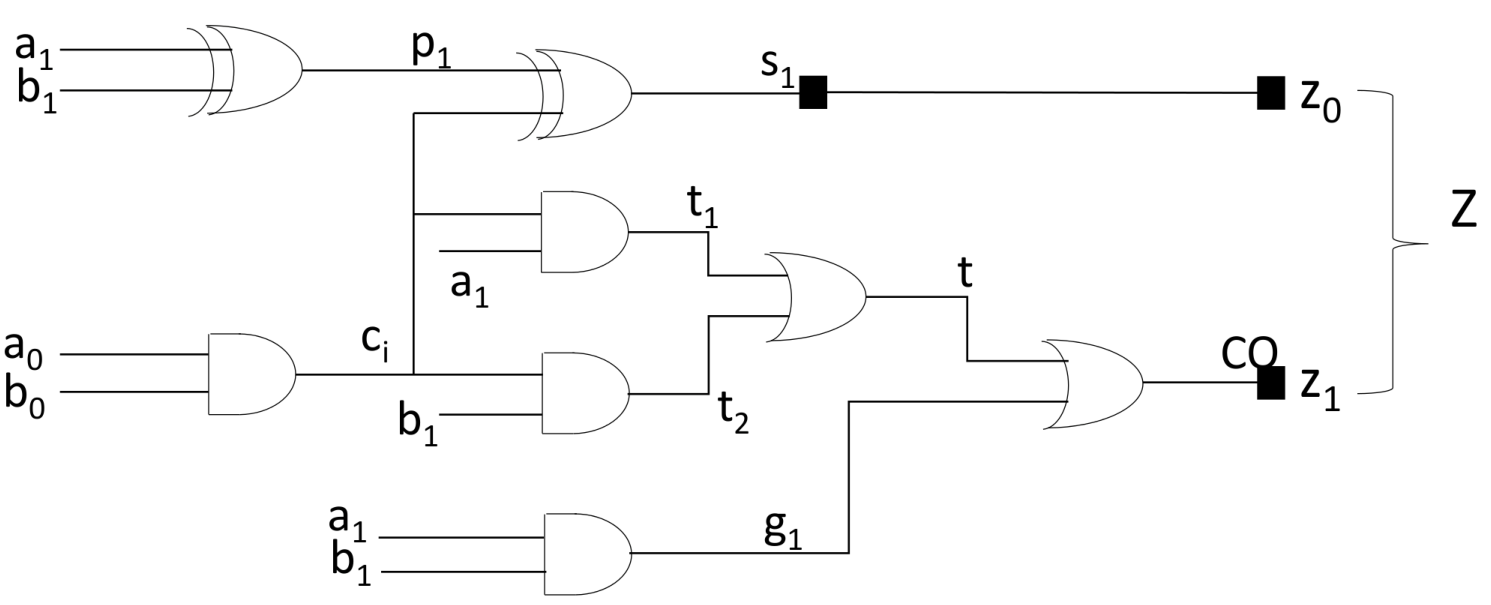
\includegraphics[width=\textwidth]{newfig/tobemapped.pdf}
% 	\end{center}
% 	\caption{An example gate-level netlist to be mapped}
% 	\label{fig:tobemapped}
% \end{figure}
% 
% Figure \ref{fig:tobemapped} shows an example circuit partition with $a_1,b_1,a_0,b_0$ as inputs and
% $Z = \{z_0,z_1\}$ as outputs. If we use elements from Galois field $\F_{2^2}$ to represent word $Z$,
% we have $Z = z_0 + \alpha\cdot z_1$.
% 
% After imposing ATO of LEX with
% $$Other\ circuit\ variables > output\ word\ Z > all\ bit\ level\ inputs$$
% on the ideal describing the partitioned circuit as well as ideal with vanishing polynomials,
% the reduced Gr\"obner basis has a single polynomial generator in the form of $Z + \Func(a_1,b_1,a_0,b_0)$.
% In this example:
% 
% \begin{itemize}
% \item Term ordering: $\{z_0,z_1,t,g_1,p_1,ci,t_1,t_2\}>Z>\{a_0,b_0,a_1,b_1$
% \item Gate description: $z_0+t+g_1+t\cdot g_1, t+t_1+t_2+t_1\cdot t_2, g_1+a_1\cdot b_1,
% 			t_1+a_1\cdot ci, t_2+b_1\cdot ci, ci+a_0\cdot b_0, z_1+p_1+ci, p_1+a_1+b_1$
% \item Word definition: $Z+z_0+z_1\cdot \alpha$
% \item Vanishing polynomial ideal $(J_0)$: $z_0^2+z_0, z_1^2+z_1, t^2+t, g_1^2+g_1, t_1^2+t_1, t_2^2+t_2, p_1^2+p_1, ci^2+ci,
% 			a_0^2+a_0, b_0^2+b_0, a_1^2+a_1, b_1^2+b_1, Z^4+Z$(since Z is a 2-bit word)
% \end{itemize}
% 
% The result is a Gr\"obner basis with single polynomial generator. The polynomial has leading term $Z$:
% $$Z+a_0\cdot b_0\cdot a_1+a_0\cdot b_0\cdot b_1+\alpha\cdot a_0\cdot b_0+a_1\cdot b_1+\alpha\cdot a_1+\alpha\cdot b_1$$
% 
% % \begin{table}
% % \centering
% % \begin{tabular}{|c|c|} \hline
% % Boolean operator & operation in $\mathbb{F}_{2}$\\ \hline
% % $\overline{a}$ & $1 + a$\\ \hline
% % $a\ and\ b$ & $ab$\\ \hline
% % $a\ or\ b$ & $a + b + ab$\\ \hline
% % $a \oplus b$ & $a + b$\\
% % \hline\end{tabular}
% % \caption{Some Boolean operators and corresponding operations in $\mathbb{F}_{2}$}
% % \label{table:booltogalois_op}
% % \end{table}
% 
% 2) {\bf Templates on Boundary Information:}
% \begin{figure}[h]
% 	\begin{center}
% 	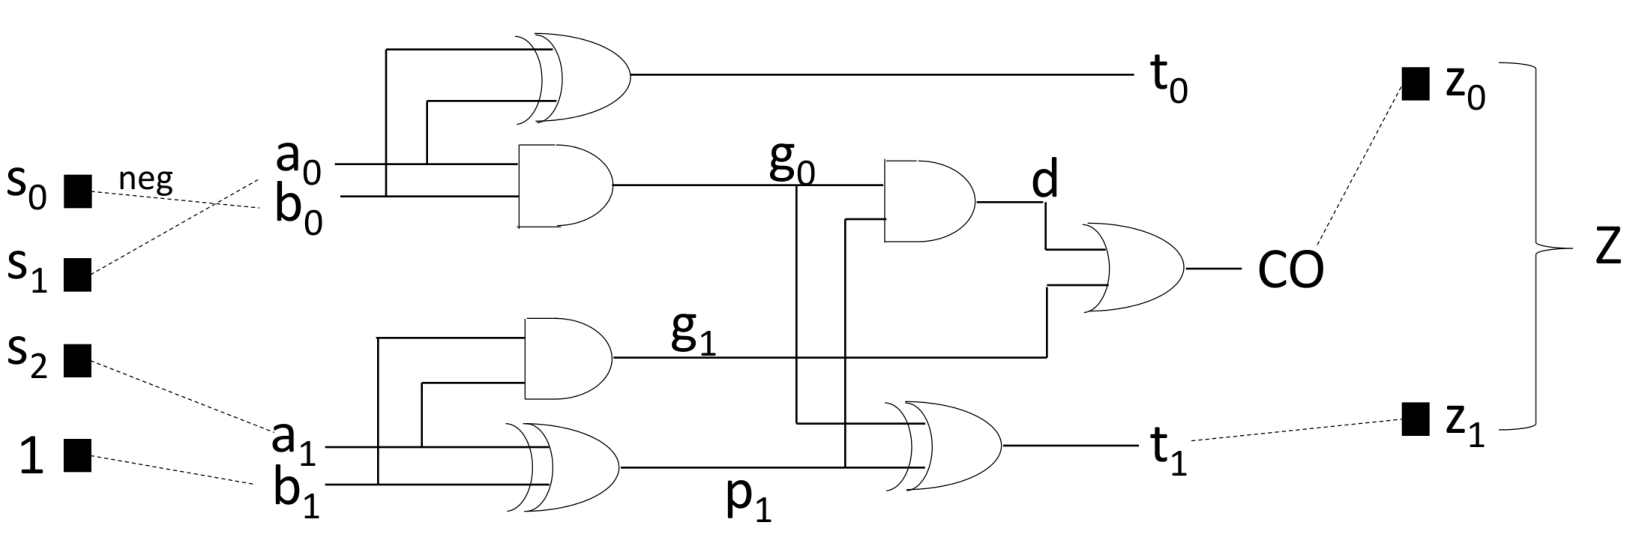
\includegraphics[width=\textwidth]{newfig/template.pdf}
% 	\end{center}
% 	\caption{Standard 2-bit adder with input/output mapping}
% 	\label{fig:template}
% \end{figure}
% 
% Figure \ref{fig:template} shows a 2-bit standard cell. It has 3 outputs mapped to 2 output pins,
% and 4 inputs mapped to 3 input pins (the rest pins are assigned to fixed 0/1 signal). Dashed connection
% lines show one possible mapping, to find out this kind of feasible mapping, we need to simulate
% all possible mappings, where the concept "template" can be used.
% 
% {\it Output template}: $z_0+c_{{t_0}{z_0}}\cdot t_0+c_{t_1z_0}\cdot t_1+c0_{CO}\cdot CO+c_{n_0}$
% 
% When $c_{n_0} = 0$, then $\{c_{t_0z_0},c_{t_1z_0},c0_{CO}\}$ equals to 1 denotes a valid mapping to corresponding output pin. 
% Conversely if $cn0 = 1$, the ``1" evaluation denotes mapping to negation of corresponding output pin.
% 
% {\it Input template}: $a_0+p_{a_0}+c0_{A_0}\cdot s_0+c1_{A_0}\cdot s_1+c2_{A_0}\cdot s_2$
% 
% When $p_{a_0} = 0$, then $\{c0_{A_0},c1_{A_0},c2_{A_0}\}$ equal to 1 denotes a valid mapping to corresponding input
% pin. Conversely if every variable in set $\{c0_{A_0},c1_{A_0},c2_{A_0}\}$ equals to 0, it denotes mapping to fixed signal ``0" (when $p_{a_0} = 1$ then
% mapping to fixed signal ``1").
% 
% With these settings, we propose an approach to perform technology mapping with boundary information:
% \begin{itemize}
% \item First, choose a set of independent wires as input pins;
% 
% \item Second, push forward input signal for a certain number of gates (depth), choose a cut set
% which fully dependent on these inputs as output pins;
% 
% \item Third, abstract a description polynomial using GB based abstraction;
% 
% \item Fourth, reduce the description polynomial with the GB we computed associated to macro block 
% and templates, obtain a remainder polynomial;
% 
% \item Last but not least, abstract all coefficients from the remainder polynomial and set up a system of equations.
% If we find a solution to this system, then the solution is a feasible mapping; no solution means we cannot make a
% feasible mapping.
% \end{itemize}